\documentclass{article}

\usepackage{import}
\usepackage{transparent}
\usepackage{xcolor}
\usepackage{tcolorbox}
\usepackage{amsmath}
\usepackage{upgreek}
\usepackage{enumitem}
\usepackage{amssymb}
\usepackage[margin=0.25in]{geometry}
\usepackage{listings}

%Commands definitions
\newcommand{\setbackgroundcolour}{\pagecolor[rgb]{0.19, 0.19, 0.19}}
\newcommand{\settextcolour}{\color[rgb]{0.87, 0.87, 0.87}}
\newcommand{\invertbackgroundtext}{\setbackgroundcolour\settextcolour}

%Command execution
%If this line is commented, then the appearance remaind as usual.
\invertbackgroundtext

\lstset{
    language=ML,
    basicstyle=\ttfamily,
    keywordstyle=\color{cyan},
    commentstyle=\color{green!70!black},
    stringstyle=\color{red},
    showstringspaces=false,
    tabsize=4,
    breaklines=true,
    breakatwhitespace=false,
}



\author{Lukasz Kopyto}
\title{Notatka na temat kopcow lewicowych}

\begin{document}
\maketitle

\section{Kopiec Drzewo lewicowe}

Kopiec jest bardzo wazna struktura danych, gdzie minimum z wszystkich elementow jest zawsze latwo i efektywnie otrzymane.

\subsection{Kopiec binarny}

W swiecie imperatywnym kopiec binarny jest czesto uzywany i czesto implementowany za pomoca tablic. Tutaj przyklad:

\begin{center}
    \begin{minipage}[h]{0.8\textwidth}
        \centering
        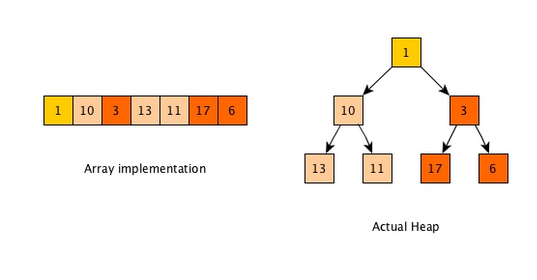
\includegraphics[width=1.0\textwidth]{ex_bin_heap.png}
    \end{minipage}    
\end{center}

Kopiec (min) po prawej stronie jest pelnym drzewem binarnym. Korzeen jest zawsze elementem minimalnym oraz rekursywnie korzen jest zawsze mniejszy od swojej dwojki dzieci. Zauwazmy, ze \textbf{dla kopca musimy utrzymac tylko czesciowy porzadek} a nie prelny tak jak w przypadku drzewa binarnego. Na przyklad 1 musi by mniejsze niz dwojka swoich dzieci, ale relacja miedzy dziecmi nie jest istotna. Zatem lewe jak i prawe dzieci moga byc 10 i 3, jak i 3 i 10. Co wiecej najwieksze dziecko - 17 moze byc w praweym poddrzewie 1, podczas gdy jego rodzic 3 jest mniejszy niz 10.

Tablicowa implementacja kopca jest calkiem fajna. Glownie uzywa ona dwoch ciekawych trickow, aby zasymulowac binarny kopiec-drzewo(binary heap tree):

\begin{tcolorbox}[colback=white!90!blue,colframe=black!35!blue,title=]

    \begin{enumerate}[label=(\arabic*)]
    \item  Jesli indeks korzenia to i, wtedy indeks jego lewego dziecka to 2*i + 1 oraz jego prawe dziecko to 2*i + 2
    \item Relacja lewego dziecka oraz prawego nie jest istotna.
    \end{enumerate}

\end{tcolorbox}

Zlozonosc czasowa operacji wynosi:

\begin{tcolorbox}[colback=white!90!blue,colframe=black!35!blue,title=]

    \begin{enumerate}[label=(\arabic*)]
        \item get\_min: $O(1)$
        \item insert: $O(logn)$
        \item delete\_min: $O(logn)$
        \item merge: $O(n)$
    \end{enumerate}
\end{tcolorbox}

Pomimo, ze merge nie jest satysfakcjonujacy, to ta struktura daje nam najbardziej efektywne uzycie pamieci w tablicy.

Jednakze, nie mozemy jej miec w czysto funkcyjnym jezyku, gdzie stan mutowalny tablic nie jest rekomendowany.

\section{Kopiec- implementacja listowa.}

Przesledzimy najpierw dwie mozliew impelementacje kopca w wersji funkcjonalnej(implementacja listowa w tej sekcji oraz implementacja przy uzyciu drzewa binarnego zaimplementowanego w nastepnej sekcji). Owe implementacje beda trywialne i nie kompletne, ale maja nas one naprowadzic na drzewa(kopce) lewicowe.

Implementacja listowa jest praktycznie zastapieniem tablic przez listy. Pomysl jest prosty:

\begin{tcolorbox}[colback=white!90!blue,colframe=black!35!blue,title=]

    \begin{enumerate}[label=(\arabic*)]
        \item Kiedy wywolujemy insert x, to liniowo porowna x z wszystkimi elementami listy i wstaw go na odpowiednie miejsce gdzie element po lewej jest mniejszy a po prawej wiekszy lub rowny od x
        \item Kiedy wywolujemy get\_min to po prostu zwracamy glowe listy.
        \item Kiedy wywolujemy delete\_min to usuwamy glowe.
        \item Kiedy wywloujemy merge to wywolujemy standardowy merge jak przy mergesort.
    \end{enumerate}

\end{tcolorbox}

Zlozonosc czasowa wynosi:

\begin{tcolorbox}[colback=white!90!blue,colframe=black!35!blue,title=]

    \begin{enumerate}[label=(\arabic*)]
        \item insert x: $O(n)$
        \item get\_min: $O(1)$
        \item delete\_min: $O(1)$
        \item merge: $O(n)$
        
    \end{enumerate}

\end{tcolorbox}

Widac ladnie na ponizszym rysunku jak to ma wygladac. Lista jest caly czas posortowana i jest to tez drzewp- zdegenerowane, z jedna galezia.
\begin{center}
    \begin{minipage}[h]{0.8\textwidth}
        \centering
        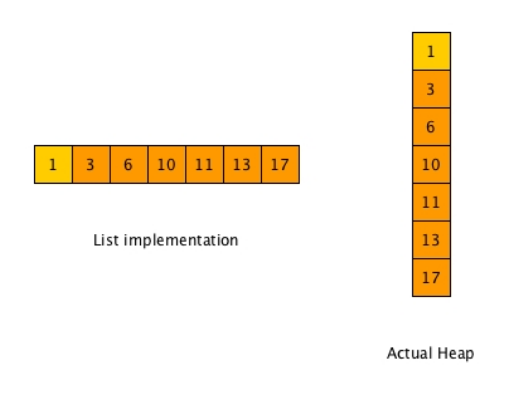
\includegraphics[width=1.0\textwidth]{heap_list.png}
    \end{minipage}    
\end{center}

Problem jest wtedy, kiedy chcemy scalic dwa kopce, czyli uzyc merge. Czas dzialania merge- $O(n)$ jest nieakceptowalny. Jest to przez to, ze musim "dokleic" cala jedna liste i wszystkie elementy musza byc uporzadkowane(totalny porzadek). Finalnie, dla kopca ten totalny porzadek nie jest wymagany i w naszej implementacji nie korzystamy z niego.

Zatem potrzebujemy conajmniej galezi zeby jakies elementy rozdzielic pomiedzy nimi i byc moze porownywanie z rodzicem bedzie szlo ominac.

\section{Kopiec binarny bez uzycia tablic}

Poniewaz kopiec binarny oparty o tablice jest tak naprawde drzewem binarnym, to bycmoze dobrym pomyslem byloby zaimplementowanie kopca binanrnego w oparciu o strukture drzewa binarnego.

Mozemy sobie zdefiniowac drzewo binarne tak o:

\begin{lstlisting}
    
    type 'a bt_heap_t = 
        | Leaf
        | Node of 'a * 'a bt_heap_t * 'a be_heap_t

\end{lstlisting}

Definicja typu jest prosta, ale problem z implementacja operacji. Spojrzmy na operacje insert jako przyklad:


\begin{center}
    \begin{minipage}[h]{0.8\textwidth}
        \centering
        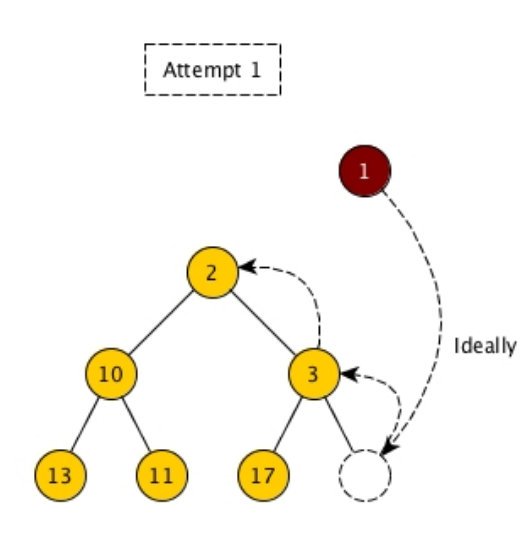
\includegraphics[width=1.0\textwidth]{insert_fst.png}
    \end{minipage}    
\end{center}

Powyzsza proba ilustruje pomysl dla tablicowej reprezentacji kopca binarnego. Jesli chcemy umiescic nowy element, to idealnie by bylo jakbysmy go mogli wsadzic na ostatnie mozliwe miejsce lub pierwsze w nowo utworzinym poziomie, jesli poprzedni jest pelny. Potem bysmy zrobili porownanie z ojcem i ewentualna zamiane. Oczywiscie nie mozemy tak zrobic w czysto drzewiastej strukturze, gdyz operacja wyszukania miejsca na wsadzenie tego nowego elementu bylaby nieefektywna. 


\begin{center}
    \begin{minipage}[h]{0.8\textwidth}
        \centering
        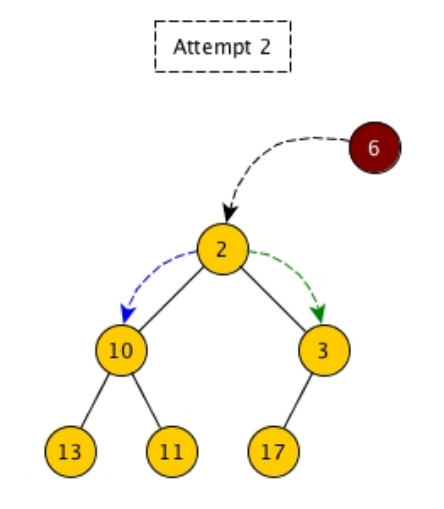
\includegraphics[width=1.0\textwidth]{insert_snd.png}
    \end{minipage}    
\end{center}

Sprobojmy zatem podejscia drugiego, top to bottom- z gory do dolu. Wsadzamy 6. Oczywiscie 2 < 6 wiec 2 zostaje i 6 idzie w dol. Ale pojawia sie pytanie, ktora galaz powinnismy wybrac idac w dol? To nie jest trywialne i powinnismy miec jakas regule na to.

\begin{center}
    \begin{minipage}[h]{0.8\textwidth}
        \centering
        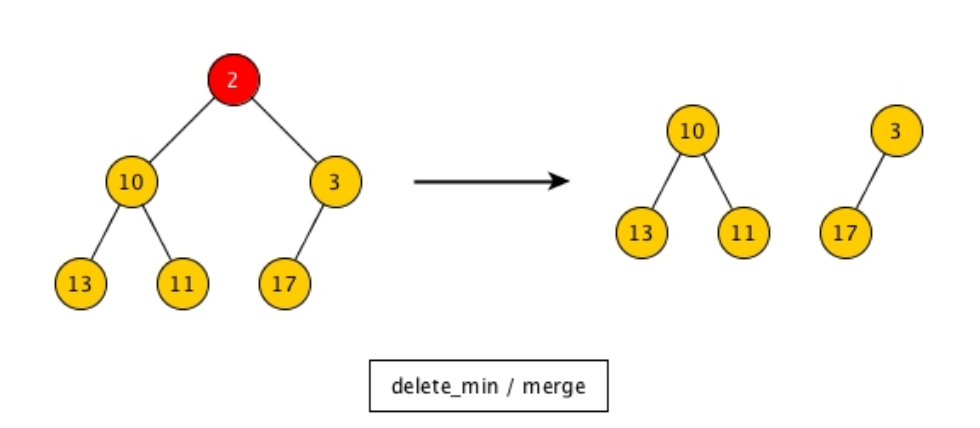
\includegraphics[width=1.0\textwidth]{delete_min.png}
    \end{minipage}    
\end{center}

Problem pojawia sie tez przy operacji delete\_min i merge, mianowicie, jesli usuniemy root(min) to otrzymamy dwa drzewa binarne. Pojawia sie pytanie, jak je scalic? Brac kazdy element z jednego drzewa i umieszczac go w drugim? Czy to byloby efektywne nawet przy dobrej implementacji inserta?

Jesli bedziemy patrzec na insert jako na merge drzewa i drzewa jednoelementowego, to problem inserta staje sie tak naprawde problemem merge. Tak jak delete\_min. \textbf{Czy zatem powinnismy skonstruowac dobrego merga aby upiec te wszystkie pieczenie przy jednym ogniu?}

Majac w glowie powyzsze pomysly i dylematy, mozemy w koncu spojrzec na drzewo lewicowe.

\section{Drzewa lewicowe}

Wszystkie watpliwosci z odpowiedzia na powyzsze pytania, maja zwiazek przede wszystkim z efektywnoscia. Zajmujemy sie drzewem. To jakie drzewo ma strutkrue oraz jak jest przetwarzane jest bardzo istotne i wplywa na efektywnosc w znaczacy sposob.

Na przyklad, na pytanie ktora galaz/sciezke wybrac podczas wywolywania metody insert, jesli bedziemy tylko szli w lewo, wtedy lewa galaz bedzie coraz bardziej wydluzala, czego skutkiem bedzie to ze zlozonosc czasowa bedzie $O(n)$.

Co wiecej podczas scalania, mamy juz podane dwa kopce binarne. Pojawia sie tu zatem zarowka, moze by wykorzystac to? Czy trzeba koniecznie niszczyc oba drzewa? Jesli moglibysmy jakos podczepic korzen jednego drzewa pod korzen drugiego drzewa, wtedy dzieci pierwszego korzenia moglyby pozostac i zadne dodatkowe operacje do nich nie sa potrzebne.

Spojrzmy zatem na drzewa lewicowe.

\subsection{Lewa strona zawsze dluzsza}

Drzewa lewicowe utrzymuja caly czas wlasnosc, taka ze lewe galezie wszystkich korzeni jako dluzsze a w najgorszym przypadku sa rowne prawym galeziom. W innych slowach, wszystkie prawe galezie wszystkich korzeni sa krotsze. To ma sens. Kiedy decydujemy sie w ktora strone isc, wiedzac ktora strona jest zawsze krotsza, to w zasadzie wiemy, w ktora strone powinnismy isc. Tak jest, poniewaz krotsze galezie znacza potencjalnie mniej wezlow i liczba mozliwych operacji jest potencjalnie mniejsza.

W celu zachowania tej wlasnosci, kazda galaz bedzie miala ranking(rank), ktory bedzie oznaczal dlugosc sciezki miedzy obecnym wezlem i najbardziej na prawo lisciem. Na przyklad:


\begin{center}
    \begin{minipage}[h]{0.8\textwidth}
        \centering
        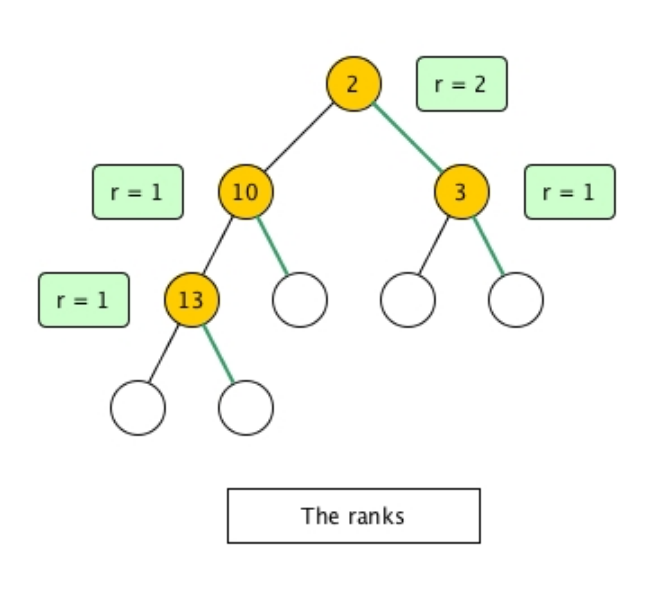
\includegraphics[width=1.0\textwidth]{ranks.png}
    \end{minipage}    
\end{center}

Sposob na to, aby utrzymywac rankingi aktualne, jest nastepujacy:

\begin{tcolorbox}[colback=white!90!blue,colframe=black!35!blue,title=]

    \begin{enumerate}[label=(\arabic*)]
        \item Zawsze \textbf{zakladamy ze rank prawego dziecka} $\leq$ \textbf{rank lewego dziecka}
        \item Zatem zawsze idziemy w prawo
        \item Jesli osiagniemy leaf(lisc), wtedy wymieniamy leaf z naszym elementem i uakutalniamy(zwiekszamy) rank wszystkich rodzicow, poczawszy od danego obecnego wezla prosto z powrotem to korzenia. Zauwazmy ze element w tym przypadku juz byc moze nie jest naszym oryginalnym elementem ktory wstawiamy(po drodze moglsmy go wymienic z elementem z innego wezla). Pozniej to wyjasnimy.
        \item Kiedy uaktualniamy rank rodzica, najpierw porownujemy, najpierw porownujemy rank lewy, \textbf{rank\_left} oraz rank prawy, \textbf{rank\_right}. Jesli \textbf{rank\_right} $<$ \textbf{rank\_left}, wtedy zamieniamy lewe dziecko z prawym dzieckiem i uaktualniamy rank rodzica jako \textbf{rank\_left + 1}. W przeciwnym przypadku uaktualniamy jako \textbf{rank\_right + 1}. 
    \end{enumerate}

\end{tcolorbox}

\vspace{10cm}

Obrazek moze to lepiej przedstawi. Budujemy drzewo lewicowe, wprowadzajac dwie nowe wartosci.

\begin{center}
    \begin{minipage}[h]{0.8\textwidth}
        \centering
        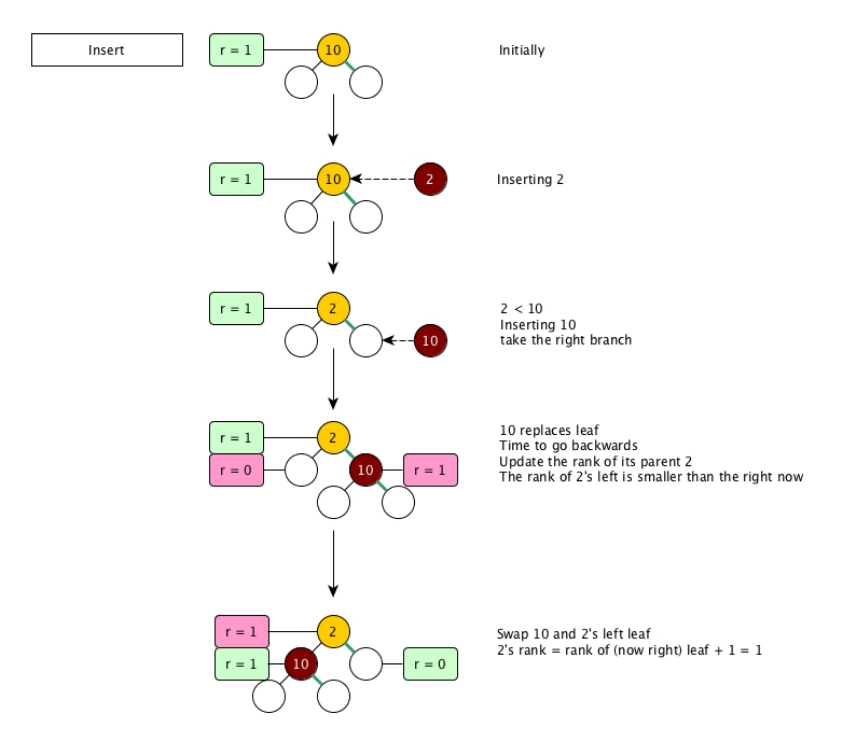
\includegraphics[width=1.0\textwidth]{insert_leftist.png}
    \end{minipage}    
\end{center}

Mozemy zauwazyc, ze przez umieszczajac wyzsze ranki z lewej strony, utrzymujemy to ze prawa galaz jest caly czas krotsza. Stad sie wziela wlasnie nazwa drzewa lewicowe, tzn potencjalnie wiecej wezlow jest po lewej stronie.

Wyzej pokazalismy na przykladzie jak dziala insert, ale mialo to charakter demonstracyjny, aby zobrazowac o co chodzi z rankiem.

W zasadzie, w drzewach lewicowych najwazniejsza operacja jest scalanie. insert to w zasadzie scalanie drzewa z singletonem drzewiastym- pojedynczy wezel z dwoma liscmi.

\subsection{Merge}

Merge jest operacja rekursyjna. Spojrzmy na pseudokod:

\begin{tcolorbox}[colback=white!90!blue,colframe=black!35!blue,title=]

    \begin{enumerate}[label=(\arabic*)]
        \item Mamy dwa drzewa do scalenia: \textbf{merge t1 t2}
        \item Porownaj dwa korzenie, jesli \textbf{k1} $>$ \textbf{k2}, to po prostu zamieniamy dwa drzewa, czyli \textbf{merge t2 t1}. Chcemy aby w lewym korzeniu byl zawsze mniejszy klucz.
        \item Poniewaz \textbf{t1} ma mniejszy klucz, jego korzen powinien zostac wynikowym korzeniem.
        \item Poniewaz prawa galaz \textbf{t1} jest zawsze krotsza od lewej, wiec scalamy prawa galaz \textbf{t1} oraz \textbf{t2}, czyli \textbf{r t2}.
        \item Jesli ktores z dwoch drzew jest lisciem to po prostu zwracamy to drugie i zaczynamy akutalizowac \textbf{rank} az do korzenia.
        \item Aktualizowanie \textbf{rank} jest takie same jak opisalismy to w przypadku procedury insert.

    \end{enumerate}

\end{tcolorbox}

\vspace{5cm}


Spojrzmy jak to wyglada na przykladzie-obrazku:

\begin{center}
    \begin{minipage}[h]{0.8\textwidth}
        \centering
        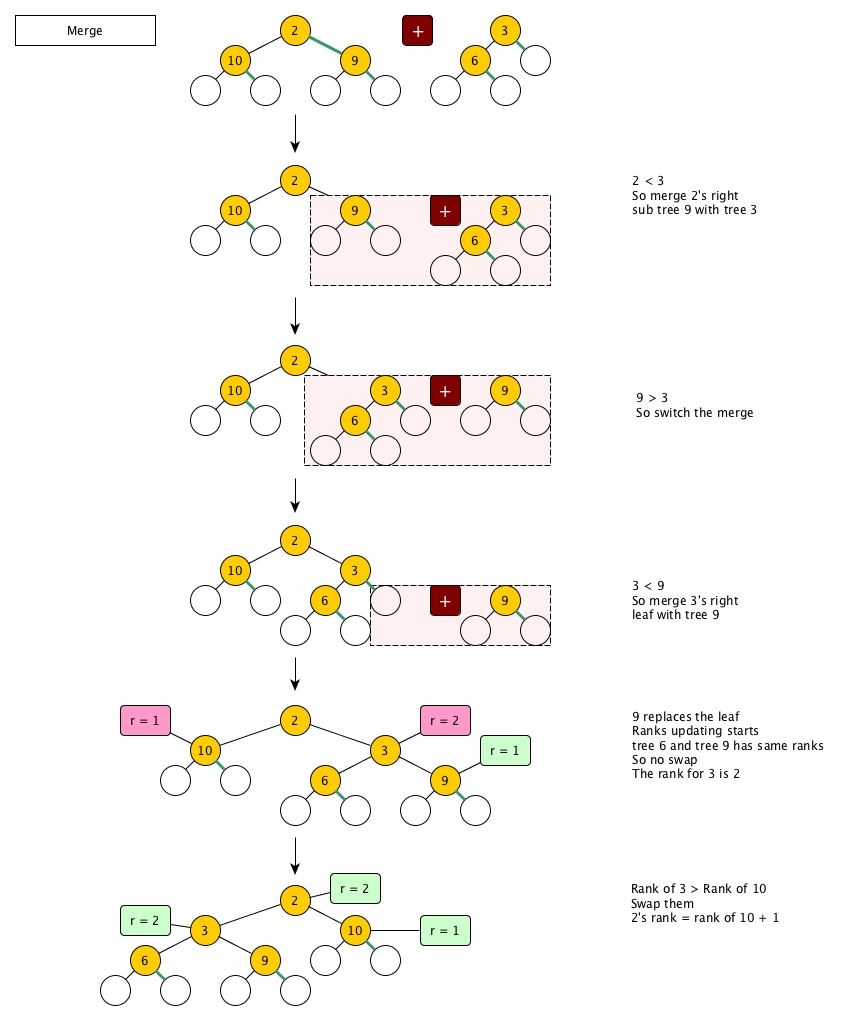
\includegraphics[width=1.0\textwidth]{left_merge.png}
    \end{minipage}    
\end{center}

Slowo komentarza:

Scalamy dwa drzewa t1 o korzeniu k1 z wartoscia 2 i t2 o korzeniu k2 z wartoscia 3: \textbf{merge t1 t2}. 

Porownujemy korzenie i k1 < k2 wiec jego korzen zostaje jako korzen wynikowy. Zatem poniewaz korzen prawa strona r korzenia k1 jest zawsze krotsza od lewej wiec scalamy teraz drzewo r o korzeniu r1 z wartoscia w nim 9 oraz drzewo t2: \textbf{merge r t2}.

Poniewaz r1 > k2, wiec zamieniamy drzewa: \textbf{merge t2 r}.

Poniewaz prawa strona t2 jest krotsza od jego lewej, wiec scalamy prawa strone drzewa t2 czyli drzewo l1 oraz drzewo r. Czyli wywolujemy \textbf{merge l1 r}

Poniewaz l1 jest lisciem, wiec zwracamy drzewo r i zaczynamy aktualizowac rank. Zatem: rank(r) = 1, rank(t2) = 2, rank(l) = 1 (l to lewe dziecko t1).

Tak jak opisane to jest opisane w metodzie insert, uakutalniajac rank rodzica sprawdzamy czy rank\_left > rank\_right, jesli tak ro zamieniamy dzieci miejscami.

W naszym przykladzie, dopiero dzieci korzenia o wartosci 2 roznia sie rankiem, czyli zamieniamy l i t2(bo t2 jest teraz nowym prawym dzieckiem)

\subsection{Kod}

typ:
\begin{lstlisting}
    type 'a leftist = 
        | Leaf
        | Node of 'a leftist * 'a * 'a leftist * int
\end{lstlisting}

podstawy:

\begin{lstlisting}
    
    let singleton k = Node (Leaf, k, Leaf, 1)

    let rank = function
        | Leaf -> 0
        | Node (_,_,_,r) -> r

\end{lstlisting}

merge:

\begin{lstlisting}

    let rec merge t1 t2 = 
        match t1,t2 with 
        | Leaf, t | t, Leaf -> t
        | Node (l, k1, r, _), Node(_, k2, _, _) ->
            if k1 > k2 
                merge t2 t1 (*zamien jesli trzeba*)
            else 
                let merged = merge r t2 in (*zawsze scalaj prawa strone*)
                let rank_left = rank l and rank_right = rank merged in 
                if rank_left >= rank_right then Node(l, k1, merged, rank_right + 1)
                else Node(merged, k1, l, rank_left + 1) (*lewy zostaje prawym przez to ze byl krotszy*)
    
\end{lstlisting}

insert, get\_min, delete\_min

\begin{lstlisting}

    let insert x t = merge (singleton x) t

    let get_min = function
        | Leaf -> failwith "Empty heap"
        | Node (_,k,_,_) -> k

    let delete_min = function
        | Leaf -> failwith "Empty heap"
        | Node (l,_,r,_) -> merge l r
    
\end{lstlisting}

Zlozonosc czasowa wynosi:

\begin{tcolorbox}[colback=white!90!blue,colframe=black!35!blue,title=]

    \begin{enumerate}[label=(\arabic*)]
        \item insert x: $O(logn)$
        \item get\_min: $O(1)$
        \item delete\_min: $O(logn)$
        \item merge: $O(logn)$
    
\end{enumerate}

\end{tcolorbox}

\end{document}
